\documentclass{article}
\usepackage{graphicx} % Required for inserting images
\usepackage[utf8]{inputenc}
\usepackage[T2A]{fontenc}
\usepackage{amsmath}
\usepackage{pgfplots}
\usepackage{longtable}
\usepackage{tabularx}
\usepackage{makecell}
\usepackage{array}
\usepackage{indentfirst}
\usepackage{icomma}
\usepackage{geometry}
\usepackage{booktabs}
\usepackage{multirow}
\usepackage{multicol}
\usepackage{float}
\usepackage{diagbox}
\usepackage{gensymb}
\geometry{a4paper, margin=1in}

\renewcommand{\figurename}{Изображение}
\renewcommand{\tablename}{Таблица}

\title{Лабораторная работа №2.05

Определение удельной теплоты кристаллизации и изменения энтропии при охлаждении олова}
\author{Топунов Антон, Z3142}
\date{07.02.2026}

\begin{document}

\maketitle
\clearpage
\section{Цели и задачи}
\subsection{Цели}
\begin{enumerate}
    \item Определение изменения энтропии при фазовом переходе первого рода на примере кристаллизации олова из расплава при его охлаждении.
    \item Определение теплоты кристаллизации олова на основе закона сохранения энергии.
\end{enumerate}
\subsection{Задачи}
\begin{enumerate}
    \item Провести прямые измерения показаний милливольтметра, фиксирующего термоЭДС
    \item Построить график зависимости температуры от времени.
    \item Вычислить удельную теплоту кристаллизации и изменение энтропии.
\end{enumerate}
\section{Теоретическое введение}

Температура окружающей среды в кельвинах:
\begin{gather*}
    T_0 = \, ^\circ t_0 - \, ^*t
\end{gather*}
где $^*t$ температура абсолютного нуля.

Мы получаем точки зависимости термоЭДС от времени $E(t)$ и переводим её с помошью таблицы в зависимость $T-T_0$ от времени.
На получившемся графике мы наблюдаем 3 участка, которые удобно анализировать в полулогарифмических осях:
Охлаждение жидкого олова:
\begin{gather*}
    \ln (T-T_0)=a+bt
\end{gather*}
Кристаллизация при постоянной температуре:
\begin{gather*}
    \ln (T_{ \text{кр}}-T_0)=const
\end{gather*}
Охлаждение твёрдого олова:
\begin{gather*}
    \ln (T-T_0) =c + Kt
\end{gather*}
Коэффициенты линейных зависимостей и их погрешности можно найти с помощью МНК.
\begin{gather*}
    \Delta K = t_{ \alpha, N}\cdot S_{ K}
\end{gather*}
где $t_{ \alpha, N}$ - коэффициент Стьюдента для доверительной вероятности $\alpha$ и количества измерений $N$,
а $S_{ K}$ - СКО, полченное в МНК.
Разность температуры кристаллизации и температуры воздуха можно найти как:
\begin{gather*}
    T_{ \text{кр}}-T_{ 0}= \frac{ \sum\limits_{i=1}^{ m}(T_i-T_{ 0})}{ m}
\end{gather*}
где суммирование идёт по точкам участка почти постоянной температуры.
А погрешность этой величины оценивается как:
\begin{gather*}
    \Delta (T_{ \text{кр}}-T_{ 0}) = \frac{ T_{ \text{max}}-T_{ \text{min}}}{ 2}
\end{gather*}
где $T_{ \text{max}}\text{ и }T_{ \text{min}}$ максимальное и минимальное значение температур на участке кристаллизации.

Ищем точки пересечения $t_1$ и $t_2$, чтобы найти $\Delta t_{ \text{кр}}=t_2 - t_1$

\begin{gather*}
    t_{ 1} = \frac{ \ln(T_{ \text{кр}}-T_0)-a}{ b}\\
    t_{ 2} = \frac{ \ln(T_{ \text{кр}}-T_0)-c}{ K}\\
\end{gather*}

Их погрешности:
\begin{gather*}
    \Delta t_1 = \sqrt{\bigg( \frac{ \Delta{(T_{\text{кр}}-T_0)}}{ b(T_{\text{кр}}-T_0)} \bigg)^2 +
        \bigg( \frac{ \Delta{a}}{ b} \bigg)^2 + 
        \bigg( \frac{ \ln(T_{ \text{кр}}-T_0)-a}{ b^2}\Delta{b} \bigg)^2}\\
    \Delta t_2 = \sqrt{\bigg( \frac{ \Delta{(T_{\text{кр}}-T_0)}}{ K(T_{\text{кр}}-T_0)} \bigg)^2 +
        \bigg( \frac{ \Delta{c}}{ K} \bigg)^2 + 
        \bigg( \frac{ \ln(T_{ \text{кр}}-T_0)-c}{ K^2}\Delta{K} \bigg)^2}
\end{gather*}

Время кристаллизации $\Delta t_{ \text{кр}}$ и его погрешность $\Delta (\Delta t_{ \text{кр}})$:
\begin{gather*}
    \Delta t_{ \text{кр}} = t_2 - t_1\\
    \Delta (\Delta t_{ \text{кр}})=\sqrt{(\Delta t_2)^2+(\Delta t_1)^2} =\\ 
        =\sqrt{\bigg( \frac{ \Delta{(T_{\text{кр}}-T_0)}}{ (T_{\text{кр}}-T_0)} \bigg)^2\cdot\bigg( \frac{ 1}{ b^2} + \frac{ 1}{ K^2}\bigg)+\bigg( \frac{ \Delta{a}}{ b} \bigg)^2 + \bigg( \frac{ \Delta{c}}{ K} \bigg)^2 +} \\
         \overline{+  
        \bigg( \frac{ \ln(T_{ \text{кр}}-T_0)-a}{ b^2}\Delta{b} \bigg)^2 + \bigg( \frac{ \ln(T_{ \text{кр}}-T_0)-c}{ K^2}\Delta{K} \bigg)^2}
\end{gather*}

Удельная теплота кристаллизации олова $\lambda$ вычисляется по формуле:
\begin{gather*}
    \lambda = -\bigg( c_{ \text{О}} + c_{ \text{А}} \cdot \frac{ M_{ \text{А}}}{ M_{ \text{О}}} \bigg)
        \cdot \Delta t_{ \text{кр}} \cdot K(T_{ \text{кр}} - T_{ 0})
\end{gather*}
где $c_{ \text{О}}$ и $c_{ \text{А}}$ - удельные теплоёмкости олова и ампулы соответственно, 
$М_{ \text{О}}$ и $М_{ \text{А}}$ - их массы,
а $K$ - угловой коэффициент, введённый раньше, как угловой коэффициент зависимости $\ln(T-T_0)$ от времени.

Температура кристаллизации:
\begin{gather*}
    T_{ \text{кр}}=(T_{ \text{кр}}-T_0) + \,^\circ t_{ 0} - \,^*t
\end{gather*}

Изменение энтропии $S_2 - S_1$ при кристаллизации олова:
\begin{gather*}
    S_{ 2} - S_{ 1} = - \frac{ \lambda{M_{ \text{О}}}}{ T_{ \text{кр}}}
\end{gather*}

Их погрешности, с учётом того, что относительная погрешность масс и теплоёмкостей олова и ампулы много меньше чем погрешнорсти экспериментальных величин:
\begin{gather*}
    \Delta \lambda = \lambda\cdot\sqrt{
        \bigg(\dfrac{\Delta(\Delta t_{ \text{кр}})}{\Delta t_{ \text{кр}}}\bigg)^2 + 
        \bigg(\dfrac{\Delta K}{K}\bigg)^2 +
        \bigg(\dfrac{\Delta (T_{ \text{кр}}-T_0)}{T_{ \text{кр}}-T_0}\bigg)^2}\\
    \quad\Delta T_{ \text{кр}}=\sqrt{(\Delta (T_{ \text{кр}}-T_0))^2+(\Delta \,^\circ t_0)^2 + (\Delta \,^* t_0)^2}\\
    \Delta (S_2 - S_1) = (S_2 - S_1)\cdot\sqrt{
        \bigg(\dfrac{\Delta \lambda }{\lambda}\bigg)^2+
        \bigg(\dfrac{\Delta M_{ \text{О}}}{M_{ \text{О}}}\bigg)^2+
        \bigg(\dfrac{\Delta T_{ кр}}{T_{ кр}}\bigg)^2
    }
\end{gather*}



\section{Схема установки}

\begin{figure}[H]
    \centering
    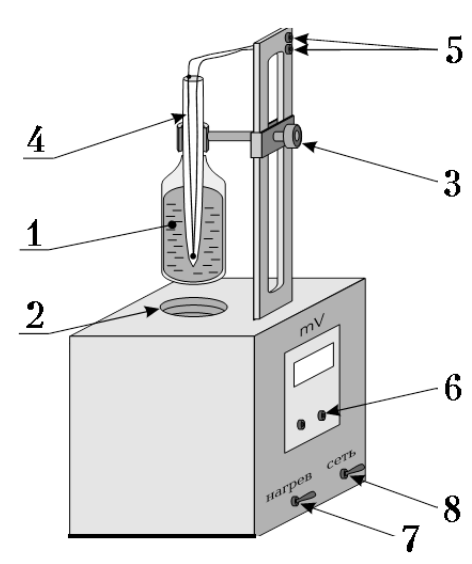
\includegraphics[width=0.75\linewidth]{Схема.png}
    \caption{Установка для лабораторной работы}
    \label{fig:placeholder}
\end{figure}

В этой лабораторной работе исследуется процесс кристаллизации олова (1),
находящегося в ампуле (4). В начале ЛР олова плавится в печке (2),
потом вынимается, закрепляетс на штативе (3), нагрев прекращается и кристаллизуется,
а потом остывает уже в твёрдом состоянии. В процессе работы с помощью термистора (5) снимается термоЭДС,
возникающее из-за разности температур в ампуле и окружающей среде. 

\section{Данные прямых измерений, табличные значения}

Масса олова:
\begin{gather*}
    M_{ \text{О}}=(70.27\pm0.01)\text{ гр}
\end{gather*}

Масса ампулы:
\begin{gather*}
    M_{ \text{А}}=(40.00\pm0.01)\text{ гр}
\end{gather*}

Удельная теплоёмкость олова:
\begin{gather*}
    c_{ \text{О}}=(0.230\pm0.001)\dfrac{\text{кДж}}{\text{кг}\cdot\text{К}}
\end{gather*}

Удельная теплоёмкость ампулы:
\begin{gather*}
    c_{ \text{А}}=(0.460\pm0.001)\dfrac{\text{кДж}}{\text{кг}\cdot\text{К}}
\end{gather*}

\begin{table}[h!]
   \centering
   \begin{tabular}{|c|c|} \hline
       $t$, с & $E$, мВ\\ \hline
        $ 0 $ & $19.2$ \\ \hline
        $30 $ & $17.7$ \\ \hline
        $60 $ & $16.4$ \\ \hline
        $90 $ & $15.2$ \\ \hline
        $120$ & $15.4$ \\ \hline
        $150$ & $15.3$ \\ \hline
        $180$ & $15.2$ \\ \hline
        $210$ & $15.3$ \\ \hline
        $240$ & $15.2$ \\ \hline
        $270$ & $15.1$ \\ \hline
        $300$ & $14.9$ \\ \hline
        $330$ & $14.6$ \\ \hline
        $360$ & $13.8$ \\ \hline
        $390$ & $12.9$ \\ \hline
        $420$ & $11.9$ \\ \hline
        $450$ & $11.1$ \\ \hline
        $480$ & $10.3$ \\ \hline
        $510$ & $ 9.7$ \\ \hline
        $540$ & $ 9.1$ \\ \hline
        $570$ & $ 8.5$ \\ \hline
        $600$ & $ 8.0$ \\ \hline
        $630$ & $ 7.4$ \\ \hline
   \end{tabular}
   \caption{Экспериментальная зависимость термоЭДС от времени}
\end{table}

Температура окружающей среды:
\begin{gather*}
    ^\circ t_0 = 22 \pm 1\, ^\circ C
\end{gather*}

Температура абсолютного нуля:
\begin{gather*}
    ^*t = -273\, ^\circ C
\end{gather*}

Коэффициенты Стьюдента для доверительной вероятности $\alpha=0.95$:
\begin{gather*}
    t_{ 0.95, 4} = 3.2\\
    t_{ 0.95, 12} = 2.3\\
\end{gather*}

\section{Расчёты и графики}


\begin{table}[H]
   \centering
   \begin{tabular}{|c|c|c|} \hline
       $t$, с & $T-T_0$, К  & $\ln(T-T_0)$\\ \hline
        $ 0 $ & $264$       & $5.576$     \\ \hline
        $30 $ & $238$       & $5.472$     \\ \hline
        $60 $ & $222$       & $5.403$     \\ \hline
        $90 $ & $208$       & $5.338$     \\ \hline
        $120$ & $210$       & $5.347$     \\ \hline
        $150$ & $209$       & $5.342$     \\ \hline
        $180$ & $208$       & $5.338$     \\ \hline
        $210$ & $209$       & $5.342$     \\ \hline
        $240$ & $208$       & $5.338$     \\ \hline
        $270$ & $207$       & $5.333$     \\ \hline
        $300$ & $204$       & $5.318$     \\ \hline
        $330$ & $200$       & $5.298$     \\ \hline
        $360$ & $191$       & $5.252$     \\ \hline
        $390$ & $179$       & $5.187$     \\ \hline
        $420$ & $167$       & $5.118$     \\ \hline
        $450$ & $156$       & $5.050$     \\ \hline
        $480$ & $146$       & $4.984$     \\ \hline
        $510$ & $138$       & $4.927$     \\ \hline
        $540$ & $130$       & $4.868$     \\ \hline
        $570$ & $122$       & $4.804$     \\ \hline
        $600$ & $115$       & $4.745$     \\ \hline
        $630$ & $107$       & $4.673$     \\ \hline
   
   \end{tabular}
   \caption{Полученная зависимость разности температур от времени и её логарифм}
\end{table}

\begin{tikzpicture}
\begin{axis}[
    width= 0.9\textwidth,
    height = 0.7\textheight,
    title style={align=center},
    title = {Зависимость разности температур от времени},
    xlabel = {$t, \text{ с}$},
    ylabel = {$T-T_0, \text{ К}$},
    minor tick num = 3,
    xmin = 0,
    xmax = 650,
    ymin = 0,
    ymax = 300,
    x tick label style = {/pgf/number format/fixed},
    y tick label style = {/pgf/number format/fixed},
    legend pos=north east,
    grid=both,
    grid style={line width=.1pt, draw=gray!10},
    major grid style={line width=.2pt,draw=gray!50},
    axis lines=middle,
    %legend style={font=\tiny},
]


\addplot[red, only marks] plot coordinates {(0, 264)
(30, 238)
(60, 222)
(90, 208)
};

\addplot[blue, only marks] plot coordinates {(90, 208)
(120, 210)
(150, 209)
(180, 208)
(210, 209)
(240, 208)
(270, 207)
};

\addplot[gray, only marks] plot coordinates {(300, 204)
(330, 200)
(360, 191)
(390, 179)
(420, 167)
(450, 156)
(480, 146)
(510, 138)
(540, 130)
(570, 122)
(600, 115)
(630, 107)};

\addplot[red, only marks, mark size=3pt] plot coordinates {(90, 208)
};

\addplot[blue, only marks] plot coordinates {(90, 208)
};

\legend{ 
	Точки процесса остывания жидкого олова,
    Точки процесса кристаллизации олова,
    Точки процесса остывания твёрдого олова
};
\end{axis}
\end{tikzpicture}


Для анализа остывания жидкого олова я выбрал значения с $t=0$ по $t=90$ включительно.

С помощью МНК коэффициенты зависимости $\ln(T-T_0) = a + bt$ получились:
\begin{gather*}
    a=5.565\\
    b = -0.0026
     \text{ с}^{ -1}\\
    \Delta a = 3.2\cdot 0.0122 \approx 0.039\\
    \Delta b = 3.2\cdot 0.00021 \approx 0.0007\text{ с}^{ -1}
\end{gather*}

Для нахождения температуры кристаллизации я выбрал значения с $t=90$ по $t=270$ включительно.

\begin{gather*}
    (T_{ \text{кр}} - T_0) = \bigg(
    \frac{ 208+210+209+208+209+208+207}{ 7}
    \bigg) \approx 208.4\text{ K}\\
    \Delta (T_{ \text{кр}} - T_0) = 0.5\cdot(210 - 207) = 1.5 \text{ К}\\
    \ln (T_{ \text{кр}} - T_{ 0})\approx5.339
\end{gather*}

Для анализа остывания твёрдого олова я выбрал значения с $t=300$ по $t=630$ включительно.
С помощью МНК коэффициенты зависимости $\ln(T-T_0) = a + bt$ получились:
\begin{gather*}
    c=5.96\\
    K = -0.00203 \text{ с}^{ -1}\\
    \Delta c = 2.3\cdot 0.019 \approx 0.04\\
    \Delta K = 2.3\cdot 0.000041 \approx 0.00009\text{ с}^{ -1}
\end{gather*}

\begin{tikzpicture}
\begin{axis}[
    width= 0.9\textwidth,
    height = 0.7\textheight,
    title style={align=center},
    title = {Зависимость логарифма разности температур от времени},
    xlabel = {$t, \text{ с}$},
    ylabel = {$\ln(T-T_0)$},
    minor tick num = 3,
    xmin = 0,
    xmax = 650,
    ymin = 4,
    ymax = 6,
    x tick label style = {/pgf/number format/fixed},
    y tick label style = {/pgf/number format/fixed},
    legend pos=south west,
    grid=both,
    grid style={line width=.1pt, draw=gray!10},
    major grid style={line width=.2pt,draw=gray!50},
    axis lines=middle,
    %legend style={font=\tiny},
]


\addplot[red, only marks] plot coordinates {(0, 5.576)
(30, 5.472)
(60, 5.403)
(90, 5.338)
};

\addplot[blue, only marks] plot coordinates {(90, 5.338)
(120, 5.347)
(150, 5.342)
(180, 5.338)
(210, 5.342)
(240, 5.338)
(270, 5.333)
};

\addplot[gray, only marks] plot coordinates {(300, 5.318)
(330, 5.298)
(360, 5.252)
(390, 5.187)
(420, 5.118)
(450, 5.050)
(480, 4.984)
(510, 4.927)
(540, 4.868)
(570, 4.804)
(600, 4.745)
(630, 4.673)};

\addplot[red, samples = 10, domain=0:650] {-0.0026*x+5.565};

\addplot[blue, samples = 10, domain=0:650] {5.339};

\addplot[gray, samples = 10, domain=0:650] {-0.00203*x+5.96};

\addplot[red, only marks, mark size=3pt] plot coordinates {(90, 5.338)
};

\addplot[blue, only marks] plot coordinates {(90, 5.338)
};

\legend{ 
	Точки процесса остывания жидкого олова,
    Точки процесса кристаллизации олова,
    Точки процесса остывания твёрдого олова,
    Аппроксимация для процесса остывания жидкого олова,
    Аппроксимация для процесса кристаллизации олова,
    Аппроксимация для процесса остывания твёрдого олова
};
\end{axis}
\end{tikzpicture}

Время процесса кристаллизации получилось:
\begin{gather*}
    \Delta t_{ \text{кр}} = t_2 - t_1 = \frac{ 5.339-5.565}{ -0.0026} - 
        \frac{ 5.339-5.96}{ -0.00203} \approx 219 \text{ с}\\
    \Delta (\Delta t_{ \text{кр}}) 
        =\sqrt{
            \bigg( \frac{ 1.5}{ 208.4} \bigg)^2\cdot\bigg( \frac{ 1}{ 0.0026^2} + \frac{ 1}{ 0.00203^2}\bigg)+
            \bigg( \frac{  0.039}{ 0.00261} \bigg)^2 +
            \bigg( \frac{ 0.04}{ 0.00203} \bigg)^2 +} \\
         \overline{+  
        \bigg( \frac{ 5.339-5.565}{ 0.0026^2} 0.0007 \bigg)^2 +
        \bigg( \frac{ 5.339-5.96}{ 0.00203^2} 0.00009 \bigg)^2}\approx37\text{ с}
\end{gather*}
    
Таким образом удельная теплота кристаллизации, температура кристаллизации и изменение энтропии:
\begin{gather*}
    \lambda = \bigg( 0.230 + 0.460 \cdot \frac{ 40.00}{ 70.27} \bigg)
        \cdot 219 \cdot 0.00203\cdot208.4\approx46 \dfrac{\text{кДж}}{\text{кг}}\\
    T_{ \text{кр}} = 208.4 + 22 + 273.15 \approx 503.6 \text{ К}\\
    S_2-S_1=- \dfrac{46\cdot10^{3} \cdot70.27\cdot10^{-3}}{503.6}=-6.4\dfrac{\text{Дж}}{\text{К}}
\end{gather*}

С учётом того, что относительные погрешности масс и удельных теплоёмкостей действительно оказались сильно меньше относительных погрешностей экспериментальных величин, можно получить погрешности: 
\begin{gather*}
    \Delta \lambda = 45.5\cdot\sqrt{
        \bigg(\dfrac{37}{219}\bigg)^2 + 
        \bigg(\dfrac{0.00009}{0.00203}\bigg)^2 +
        \bigg(\dfrac{1.5}{208.4}\bigg)^2}\approx8 \dfrac{\text{кДж}}{\text{кг}}\\
    \Delta T_{ \text{кр}}=\sqrt{(1.5)^2+(1)^2 + (0.005)^2}\approx1.8\text{ К}\\
    \Delta (S_2 - S_1) = 6.41\cdot\sqrt{
        \bigg(\dfrac{8}{46}\bigg)^2+
        \bigg(\dfrac{0.01}{70 .27}\bigg)^2+
        \bigg(\dfrac{1.8}{503.6}\bigg)^2}\approx1.1\dfrac{\text{Дж}}{\text{К}}
\end{gather*}

\section{Результаты и выводы}

Полученное значене удельной теплоты кристаллизации олова $\lambda = (46\pm8) \frac{ \text{ кДж}} {\text{кг}}$
близка к реальному значения $\lambda_{ \text{табл}}=60.7 \frac{ \text{кДж}}{ \text{кг}}$, но всё-же меньше.
Это могло получиться из-за того, что реальная длительность процесса кристаллизации была больше чем получанная мной
т.к. процесс проходил не при постоянной температуре, а точек, полученных при процессе остывания жидкого олова недостаточно,
чтобы получить правильную зависимость и нужное время начала процесса.

Температура кристаллизации получилась $T_{ \text{кр}}=(503.6\pm1.8)\text{ К}$,
что совпадает с табличной температурой кристаллизации $T_{ \text{табл}}=(505\pm1)\text{ К}$.
 
Изменение энтропии получилось $S_2 - S_1 = (-6.4 \pm 1.1)\dfrac{\text{Дж}}{\text{К}}$,
что меньше ожидаемого (теоретическое значение $S_2 - S_1\approx$-8.4), как следствие меньшей удельной теплоты кристаллизации, но всё равно достаточно близко. 

\newpage

\begin{figure}[H]
    \centering
    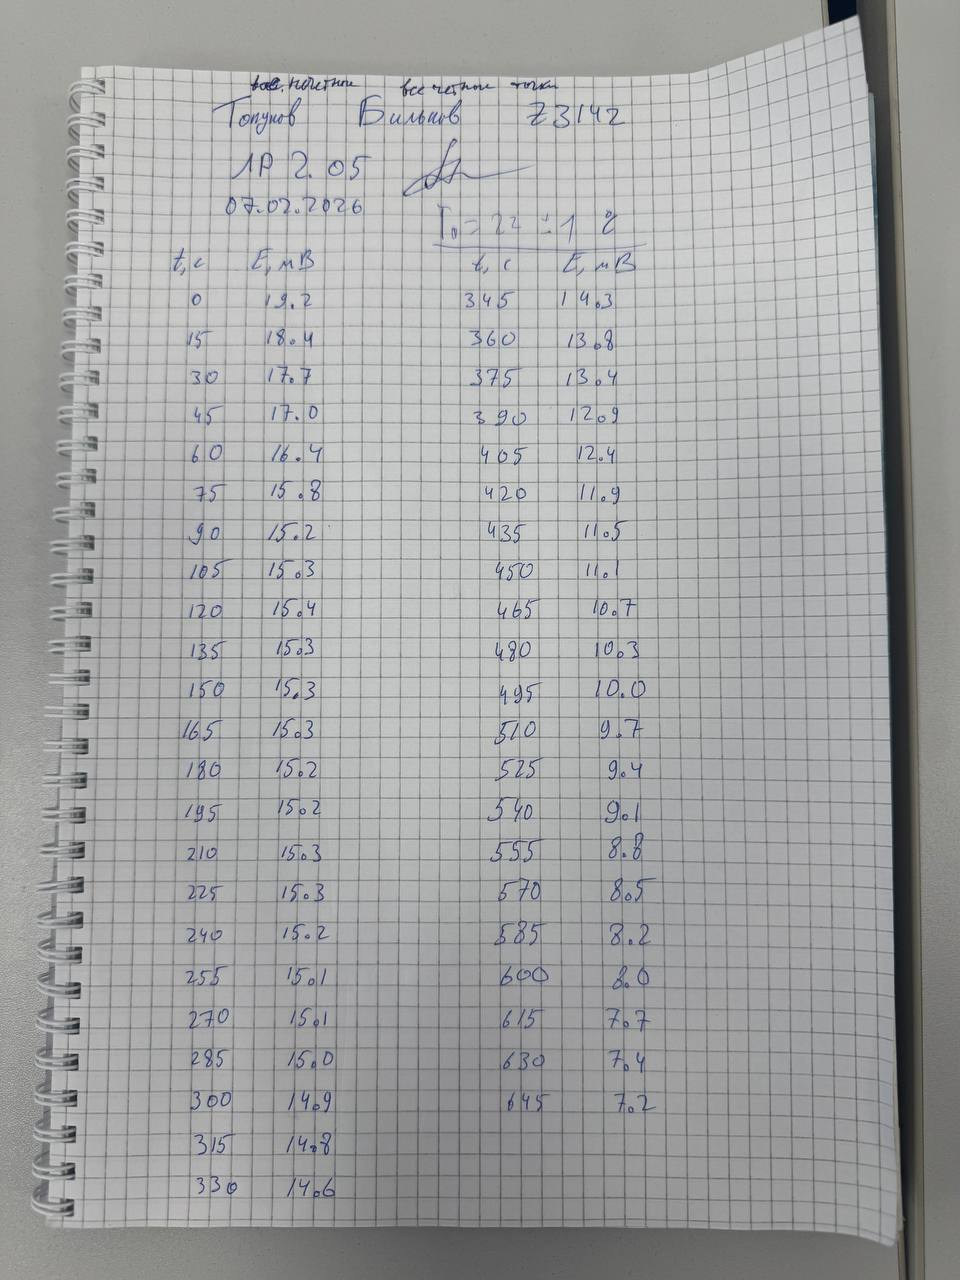
\includegraphics[width=1\linewidth]{измерения.jpg}
    \caption{Данные прямых измерений}
    \label{fig:placeholder}
\end{figure}


\end{document}